

% = Counter
\newcounter{evncount}[chapter]
\setcounter{evncount}{0}
\renewcommand{\theevncount}{\thechapter.\arabic{evncount}}
\renewcommand{\theequation}{\thechapter-\arabic{equation}}


% = Eksempler = example =
\newenvironment{example}[1][]{
	\refstepcounter{evncount}
	\setlength{\obsl}{\textwidth-1.2cm-13.2pt-9pt} % fix width of the info envirnment%
	\def\FrameCommand{ 
		\textcolor{mingroenstreg}{\vrule width 4pt} 
		\hspace{5pt} 
	}%
	\MakeFramed{\advance\hsize-\width \FrameRestore}%
	\needspace{3\baselineskip}
	\titlegraphic{mingroen}
	\textcolor{mingroen}{
		\th{Eksempel \theevncount \hspace*{5mm} #1}
	} 
	\vspace*{3mm}%
	\begin{small}
	\par
}
{
	\end{small}
	\endMakeFramed
}


% = Opgaver = exercise =
\newenvironment{exercise}[1][]{
	\refstepcounter{evncount}
	\setlength{\obsl}{\textwidth-1.2cm-13.2pt-9pt}% fix width of the info envirnment%
	\def\FrameCommand{
		\textcolor{minorangestreg}{\vrule width 4pt}
		\hspace{5pt}
	}%
	\MakeFramed{\advance\hsize-\width \FrameRestore}%
	\needspace{3\baselineskip}
	\titlegraphic{minorange}
	\textcolor{minorange}{
		\th{Opgave \theevncount \hspace*{5mm} #1}
	} 
	\vspace*{3mm}%
	\begin{small}
	\par
}
{
	\end{small}
	\endMakeFramed
}


% = Bevis
\newenvironment{bevis}{
	\setlength{\obsl}{\textwidth-1.2cm-13.2pt-9pt} % fix width of the info envirnment%
	\def\FrameCommand{
		\textcolor{mingraastreg}{\vrule width 4pt} 
		\hspace{5pt}
	}%
	\MakeFramed{\advance\hsize-\width \FrameRestore}%
	\needspace{3\baselineskip}
	\titlegraphic{black}
	\textcolor{black}{
		\th{Bevis}
	}
	\vspace*{3mm}%
	\begin{small}
	\par
}
{
	\bevisslut 
	\end{small}
	\endMakeFramed
}


% = Definition =
\newenvironment{definition}[1][]{
	\vspace{4mm}
	\pagebreak[1]
	\setlength{\obsl}{\textwidth-1.2cm-2\FrameSep-13.2pt}%
	\def\FrameCommand{
		\fboxsep=\FrameSep\fcolorbox{minblaa}{thmbackground}
	}
	\begin{minipage}{\textwidth}
	\MakeFramed{\advance\hsize-\width\FrameRestore}
	\refstepcounter{evncount}
	\titlegraphic{minblaa}
	\textcolor{minmblaa}{
		\th{Definition \theevncount \hspace*{5mm} #1}
	}
	\vspace*{3mm}
	\par
}
{
	\endMakeFramed 
	\end{minipage}
	\vspace{4mm}
}


% = Theorem =
\newenvironment{theorem}[1][]{
	\vspace{4mm}
	\pagebreak[1]%
	\setlength{\obsl}{\textwidth-1.2cm-2\FrameSep-13.2pt}%
	\def\FrameCommand{
		\fboxsep=\FrameSep\fcolorbox{minblaa}{thmbackground}
	}%
	\begin{minipage}{\textwidth}
	\MakeFramed{\advance\hsize-\width\FrameRestore}%
	\refstepcounter{evncount}
	\titlegraphic{minblaa}
	\textcolor{minmblaa}{
		\th{S�tning \theevncount \hspace*{5mm} #1}
	}
	\vspace*{3mm}
	\par
}
{
	\endMakeFramed 
	\end{minipage}
	\vspace{4mm}
}


% = Lemma =
\newenvironment{lemma}[1][]{
	\vspace{4mm}
	\pagebreak[1]
	\setlength{\obsl}{\textwidth-1.2cm-2\FrameSep-13.2pt}%
	\def\FrameCommand{
		\fboxsep=\FrameSep \fcolorbox{minblaa}{thmbackground}
	}
	\begin{minipage}{\textwidth} 
	\MakeFramed{\advance\hsize-\width \FrameRestore}
	\refstepcounter{evncount}
	\titlegraphic{minblaa}
	\textcolor{minmblaa}{
		\th{Hj�lpes�tning \theevncount \hspace*{5mm} #1}
	}
	\vspace*{3mm}
	\par
}
{
	\endMakeFramed 
	\end{minipage}
	\vspace{4mm}
}


% = Corollary =
\newenvironment{corollary}[1][]{
	\vspace{4mm}
	\pagebreak[1]
	\setlength{\obsl}{\textwidth-1.2cm-2\FrameSep-13.2pt}%
	\def\FrameCommand{
		\fboxsep=\FrameSep \fcolorbox{minblaa}{thmbackground}
	}
	\begin{minipage}{\textwidth} 
	\MakeFramed{\advance\hsize-\width \FrameRestore}
	\refstepcounter{evncount}
	\titlegraphic{minblaa}
	\textcolor{minmblaa}{
		\th{F�lges�tning \theevncount \hspace*{5mm} #1}
	}
	\vspace*{3mm}
	\par
}
{
	\endMakeFramed 
	\end{minipage}
	\vspace{4mm}
}


% = Metode = method
\newenvironment{method}[1][]{
	\vspace{4mm}
	\pagebreak[1]
	\setlength{\obsl}{\textwidth-1.2cm-2\FrameSep-13.2pt}%
	\def\FrameCommand{
		\fboxsep=\FrameSep \fcolorbox{black}{hvadbackground}
	}
	\begin{minipage}{\textwidth} 
	\MakeFramed{\advance\hsize-\width \FrameRestore}
	\refstepcounter{evncount}
	\titlegraphic{black}
	\textcolor{black}{
		\th{Metode \theevncount \hspace*{5mm} #1}
	}
	\vspace*{3mm}
	\par
}
{
	\endMakeFramed
	\end{minipage}
	\vspace{4mm}
}


% = Forklaring = explain =
\newenvironment{explain}[1][]{
	\vspace{4mm}
	\pagebreak[1]
	\setlength{\obsl}{\textwidth-1.2cm-2\FrameSep-13.2pt}%
	\def\FrameCommand{
		\fboxsep=\FrameSep \fcolorbox{black}{hvadbackground}
	}
	\MakeFramed{\advance\hsize-\width \FrameRestore}
	\refstepcounter{evncount}
	\titlegraphic{black}
	\textcolor{black}{
		\th{Forklaring \theevncount \hspace*{5mm} #1}
	}
	\vspace*{3mm}
	\par
}
{
	\endMakeFramed
	\vspace{4mm}
}


% = Bem�rkning = remark =
\newenvironment{remark}[1][]{
	\vspace{4mm}
	\pagebreak[1]
	\setlength{\obsl}{\textwidth-1.2cm-2\FrameSep-13.2pt}%
	\def\FrameCommand{
		\fboxsep=\FrameSep \fcolorbox{black}{hvadbackground}
	}
	\begin{minipage}{\textwidth} 
	\MakeFramed{\advance\hsize-\width \FrameRestore}
	\refstepcounter{evncount}
	\titlegraphic{black}
	\textcolor{black}{
		\th{Bem�rkning \theevncount \hspace*{5mm} #1}
	}
	\vspace*{3mm}
	\par
}
{
	\endMakeFramed 
	\end{minipage}
	\vspace{4mm}
}







% = OBS! = obs =
\newenvironment{obs}{\vspace{4mm}\par%
\begin{tabular}{m{1.2cm}<{\hspace*{2mm}}@{}|m{\obsl}@{}}\hspace*{-4pt}\raggedleft
\includegraphics[width=1.1cm]{../Strukturfiler/FIGS/Alert01} & \begin{minipage}{\obsl}}{\end{minipage}\\ \end{tabular}\vspace{4mm}\par}


% = INFO = info =
\newenvironment{info}{\vspace{4mm}\par%
\begin{tabular}{m{1.2cm}<{\hspace*{2mm}}@{}|m{\obsl}@{}}\hspace*{-4pt}\raggedleft
\includegraphics[width=1.1cm]{../Strukturfiler/FIGS/Info01} & \begin{minipage}{\obsl}}{\end{minipage}\\ \end{tabular}\vspace{4mm}\par}


% = THINK= think =
\newenvironment{think}{\vspace{4mm}\par%
\begin{tabular}{m{1.2cm}<{\hspace*{2mm}}@{}|m{\obsl}@{}}\hspace*{-4pt}\raggedleft
\includegraphics[width=0.7cm]{../Strukturfiler/FIGS/ChessPiece} & \begin{minipage}{\obsl}}{\end{minipage}\\ \end{tabular}\vspace{4mm}\par}


% = AHA= aha =
\newenvironment{aha}{\vspace{4mm}\par%
\begin{tabular}{m{1.2cm}<{\hspace*{2mm}}@{}|m{\obsl}@{}}\hspace*{-4pt}\raggedleft
\includegraphics[width=1.1cm]{../Strukturfiler/FIGS/Think} & \begin{minipage}{\obsl}}{\end{minipage}\\ \end{tabular}\vspace{4mm}\par}


% = BUILDUP= build =
\newenvironment{build}{\vspace{4mm}\par%
\begin{tabular}{m{1.2cm}<{\hspace*{2mm}}@{}|m{\obsl}@{}}\hspace*{-4pt}\raggedleft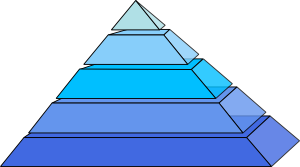
\includegraphics[width=1.1cm]{../Strukturfiler/FIGS/BluePyramid} & \begin{minipage}{\obsl}}{\end{minipage}\\ \end{tabular}\vspace{4mm}\newline}


% = Foruds�tning = basis
\newenvironment{basis}{\begin{flushleft} \begin{itshape} }{\end{itshape} \end{flushleft}}


% = Opsummering =
\newenvironment{summary}{\clearpage\pagecolor{sumgul}\section{Opsummering}}{\newpage\pagecolor{white}}











% = Counter
\newcounter{opgavecount}[section]
\setcounter{opgavecount}{0}
\newcounter{spgcount}[opgavecount]
\setcounter{spgcount}{0}
\renewcommand{\thespgcount}{\alph{spgcount})}



% = EXERCISE = (DIVIDER)

\newcommand{\exercisebegin}[1][]{\bigskip\needspace{3\baselineskip}\refstepcounter{opgavecount}\titlegraphic{mingroen}\textcolor{mingroen}{\th{Opgave \theopgavecount \hspace*{1cm} #1}}\medskip\par}

% = QUIZEXERCISE = (DIVIDER)

\newcommand{\quizexercisebegin}[1][]{\bigskip\needspace{3\baselineskip}\refstepcounter{opgavecount}\titlegraphic{mingroen}\textcolor{mingroen}{\th{Quiz-Opgave \theopgavecount \hspace*{1cm} #1}}\medskip\par}

% = QUESTION =

\newenvironment{question}{\refstepcounter{spgcount}\begin{itemize}\item[\thespgcount]}{\end{itemize}\hspace*{\fill}}

% = VINK =

\newenvironment{vink}{\begin{tabular}{m{.9cm}<{\hspace*{2mm}}@{}|m{\obsl}@{}}\hspace*{-4pt}\raggedleft
\includegraphics[width=.9cm]{../Strukturfiler/FIGS/Think} & \begin{minipage}{\obsl}}{\end{minipage}\\ \end{tabular}\medskip\\}
	
% = FACIT =

\newenvironment{facit}{\begin{tabular}{m{.9cm}<{\hspace*{2mm}}@{}|m{\obsl}@{}}\hspace*{-4pt}\raggedleft
\includegraphics[width=.9cm]{../Strukturfiler/FIGS/Check} & \begin{minipage}{\obsl}}{\end{minipage}\\ \end{tabular}\medskip\\}








\newcommand{\afsnit}[1]{\bigskip\th{\titlegraphic{mingroen}\textcolor{mingroen}{#1}} \\ \rule[7pt]{.4\textwidth}{1pt} \vspace*{-2.5mm}\par}

% (DIVIDER):
\newcommand{\ugedagdatotitel}[4]{\pagebreak[4]\section{Semesteruge #1 -- #2 Dag \hspace*{1mm} (#3)} \vspace*{-4mm} \rule[5pt]{\textwidth}{1pt}\vspace*{-2.5mm} \begin{center}\large{\th{#4}}\end{center} \fancyhead[C]{\th{Semesteruge #1}}}

\newenvironment{skema}[1]{\definecolor{shadecolor}{rgb}{0.96,.98, 1.0} \setlength{\FrameSep}{6pt} \renewcommand{\FrameHeightAdjust}{10pt} \vspace*{-4pt}\begin{shaded} \begin{tabular}{#1}}{\end{tabular} \end{shaded} \vspace*{-7pt}}

